\documentclass[11pt,a4paper]{article}
\usepackage[margin=2.4cm]{geometry}
\usepackage{amsmath,amssymb,graphicx,booktabs}
\usepackage[colorlinks,linkcolor=blue,urlcolor=blue]{hyperref}

\renewcommand{\d}{\,\mathrm{d}}
\newcommand{\e}{\mathrm{e}}
\newcommand{\E}{\mathrm{E}}
\newcommand{\skappa}{\tilde\kappa}
\newcommand{\MC}{\texttt{MCIQ4.cpp}}
\newcommand{\ISIF}{\texttt{IQ4.cpp}}

\title{\bf A Monte Carlo method for the stratified VRTE\\[2pt]
\large system (4.9)--(4.10)--(4.11) of Chapter 4}
\author{O. Pironneau}
\date{\today}

\begin{document}
\maketitle

\begin{abstract}\noindent
The polarized radiative transfer equations of a stratified atmosphere, coupled with the
radiative equilibrium equation for the temperature, are solved by a Monte Carlo method.
The key point is that in the variables $I_l,I_r$ the scattering kernel is a
\emph{probability density}, so that no negative weight is needed; the polarization is
then carried by a two-component weight which is updated deterministically, which removes
the sampling noise on $Q$. The method needs no closure and no $\E_n$ quadrature. It is
verified against an independent discrete ordinates solver (0.05\% on $J_0$) and against
the ISIF solver \ISIF\ ($0.27\,^\circ$C r.m.s.\ on the temperature). On the test case of
Chapter~4 a 20\% increase of $\kappa_\nu$ in the $14$--$18\,\mu$m band of CO$_2$ warms the
ground by $0.97\,^\circ$C and cools the tropopause by $1.35\,^\circ$C, against $+0.93$ and
$-1.31\,^\circ$C for ISIF on the same grid.
\end{abstract}

\section{The problem}
For $z\in(0,Z)$, $\mu\in(-1,1)$ and all frequencies $\nu$, with
$P_2(\mu)=\frac12(3\mu^2-1)$, $\sigma_s=\kappa_\nu a_s$, $\sigma_a=\kappa_\nu(1-a_s)$,
\begin{align}\label{eq:lq0}
\mu\partial_z I+\kappa_\nu I&=\sigma_aB_\nu(T)+\frac{\sigma_s}2\int_{-1}^1 I\d\mu'
+\frac{\beta\sigma_s}4P_2(\mu)\int_{-1}^1[P_2I-(1-P_2)Q]\d\mu',\notag\\
\mu\partial_z Q+\kappa_\nu Q&=-\frac{\beta\sigma_s}4\big(1-P_2(\mu)\big)\int_{-1}^1[P_2I-(1-P_2)Q]\d\mu',
\end{align}
with the boundary conditions (a Lambert ground with albedo, a collimated sun)
\begin{align}\label{eq:bc0}
&I(0,\mu)=c'_eB_\nu(T_e)\mu+q_0\int_{-1}^0\mu I(0,\mu)\d\mu,\quad Q(0,\mu)=0,&&\mu>0,\notag\\
&I(Z,\mu)=c_sB_\nu(T_s)\delta(\mu+\mu_s),\quad\ \ \, Q(Z,\mu)=0,&&\mu<0,
\end{align}
and the temperature given at each altitude by the radiative equilibrium
\begin{align}\label{eq:fort0}
\int_{\mathbb{R}_+}\sigma_a\Big(B_\nu(T)-\tfrac12\int_{-1}^1I\d\mu\Big)\d\nu=0 .
\end{align}
Two difficulties: the integral terms couple $I$ and $Q$ at every altitude, and
\eqref{eq:fort0} couples all the frequencies through $T(z)$.

\section{The method}

\subsection{An equivalent system whose kernel is a probability density}
Monte Carlo transport \cite{hammersley,spanier,marchuk,mayer} needs a nonnegative kernel,
which \eqref{eq:lq0} does not have: the source of
$Q$ is a negative quantity. In the variables of (4.8),
\[
I_l=\tfrac12(I+Q),\qquad I_r=\tfrac12(I-Q),
\]
the system becomes, for $p\in\{l,r\}$,
\begin{align}\label{eq:lr}
\mu\partial_z I_p+\kappa_\nu I_p=\sigma_s\sum_{p'}\int_{-1}^1K_{pp'}(\mu,\mu')I_{p'}(\mu')\d\mu'
+\tfrac12\sigma_aB_\nu(T),
\end{align}
with, writing $b=\tfrac{3\beta}8$ and $u=\tfrac{1-\beta}4$,
\begin{equation}\label{eq:K}
\begin{aligned}
K_{ll}&=b\big[2(1-\mu^2)(1-\mu'^2)+\mu^2\mu'^2\big]+u, &\qquad K_{lr}&=b\,\mu^2+u,\\
K_{rl}&=b\,\mu'^2+u,&\qquad K_{rr}&=b+u .
\end{aligned}
\end{equation}
This form has the two properties a random walk requires:
\begin{equation}\label{eq:proba}
K_{pp'}(\mu,\mu')\ge0 \quad\text{and}\quad
\sum_{p}\int_{-1}^1K_{pp'}(\mu,\mu')\d\mu=1,\qquad p'=l,r .
\end{equation}
The second one is a one line computation, with $\int_{-1}^1(1-\mu^2)\d\mu=\frac43$ and
$\int_{-1}^1\mu^2\d\mu=\frac23$: the terms in $\mu'^2$ cancel and there remains
$\frac83b+4u=\beta+(1-\beta)=1$. Hence $K_{\cdot p'}(\cdot,\mu')$ is the probability
density of the direction \emph{and} of the state of polarization after a collision; the
scattering conserves the energy exactly and an analog Monte Carlo is possible. (That
\eqref{eq:lr}--\eqref{eq:K} is \eqref{eq:lq0} is checked by taking the sum and the
difference of the two equations, with $\int P_2I=\frac12(3J_2-J_0)$ etc.)

\subsection{The random walk}
A photon carries an altitude $z$, a direction cosine $\mu$ and \emph{a pair of weights}
$(w_l,w_r)$; it represents $w_l+w_r$ units of $I$ and $w_l-w_r$ units of $Q$. Between two
collisions the optical depth travelled is $-\log U$, $U$ uniform in $(0,1)$; $\kappa_\nu$
being piecewise constant in $z$, the walk from cell to cell is exact. At a collision the
absorbed part $(1-a_s)(w_l+w_r)$ is scored and the weights are multiplied by $a_s$
(implicit capture, with Russian roulette below $10^{-4}$ of the initial weight).

At the collision only the \emph{direction} is sampled. Let
$c_p(\mu)=K_{pl}(\mu,\mu')w_l+K_{pr}(\mu,\mu')w_r$ be the intensity scattered in the
direction $\mu$ with the state $p$. By \eqref{eq:proba}, $\int\sum_pc_p\d\mu=w_l+w_r$, so
\[
h(\mu)=\frac{c_l(\mu)+c_r(\mu)}{w_l+w_r}
=\frac{A(1-\mu^2)+B\mu^2+C}{w_l+w_r}
\]
is a probability density, with $A=2b(1-\mu'^2)w_l$, $B=b(\mu'^2w_l+w_r)$ and
$C=(b\mu'^2+2u)w_l+(b+2u)w_r$. One samples $\mu$ from $h$, a mixture of three elementary
densities of masses $\frac43A$, $\frac23B$ and $2C$, inverted in closed form:
\[
\tfrac34(1-\mu^2):\ \mu=2\cos\frac{\arccos(1-2U)+4\pi}{3},\qquad
\tfrac32\mu^2:\ \mu=\pm U^{1/3},\qquad
\tfrac12:\ \mu=2U-1,
\]
and the weights are then updated \emph{deterministically},
\begin{equation}\label{eq:wsplit}
w_p\ \longleftarrow\ (w_l+w_r)\,\frac{c_p(\mu)}{c_l(\mu)+c_r(\mu)},\qquad p=l,r .
\end{equation}
The total weight $w_l+w_r$ is therefore conserved exactly at every collision, and the
polarization carries \emph{no} sampling noise. This matters: $Q$ is 1 to 2\% of $I$, so
drawing a random state $l$ or $r$ at each collision --- the obvious analog scheme --- makes
$Q$ a difference of two nearly equal random sums and needs some $10^4$ times more photons
for the same accuracy. We measured a factor $50$ on the error of $Q$ for the same cost.

\subsection{Sources and boundary conditions}
A weight is a current (an energy per unit area), so a boundary datum $g(\mu)$ emits
$\int\mu g\d\mu$ and a volume source $q$ of \eqref{eq:lq0} emits $2q$ per unit length.
The three sources and their sampling are
\[
\begin{array}{lll}
\text{sun, } z=Z: & \mu_sc_sB_\nu(T_s), & \mu=-\mu_s,\\[2pt]
\text{ground, } z=0: & \tfrac13c'_eB_\nu(T_e), & \mu=U^{1/3},\\[2pt]
\text{air, } z\in(0,Z): & 2\sigma_aB_\nu(T(z)), & \mu=2U-1,
\end{array}
\]
all three unpolarized, i.e.\ $w_l=w_r$. The Lambert condition of \eqref{eq:bc0} is a
reflection: the reflected radiance $q_0\int_{-1}^0\mu I\d\mu$ is isotropic, so the ground
returns the fraction $|q_0|/2$ of the current it receives, in the direction $\mu=\sqrt U$
and unpolarized; the rest is absorbed. The constant $c_0$ of (4.13) is obtained as a
by-product, $c_0=|q_0|\times$ (current received by the ground).

\subsection{Estimators}
Track lengths give, in each cell and for $q=0,2$,
\[
J_q(z)=\frac1{2\Delta z}\sum (w_l+w_r)\,\ell\,\mu^q,\qquad
K_q(z)=\frac1{2\Delta z}\sum (w_l-w_r)\,\ell\,\mu^q,
\]
the sums being over the portions of trajectory of length $\ell$ inside the cell; the same
sums binned in $\mu$ give the surfaces $I(z,\mu)$ and $Q(z,\mu)$. The intensities leaving
the atmosphere are obtained by a next event estimator, which is much smoother than
counting the escaping photons: each collision at $z$ contributes
$c_p(\mu)\e^{-\skappa(z,Z)/\mu}/\mu$ to $I_p(Z,\mu)$, $\mu>0$. Finally the uncollided
sunlight is not sampled --- it is a Dirac --- but added analytically,
$J_q\mathrel{+}=\frac12\mu_s^qc_sB_\nu(T_s)\e^{-\skappa(z,Z)/\mu_s}$, which also removes
its variance.

\subsection{Coupling with the temperature}
For a given $T(z)$ the Monte Carlo solves the transport problem, \emph{scattering
included}, in a single pass: unlike ISIF it does not iterate on the source. Only
\eqref{eq:fort0} needs an outer loop: $T$ is initialized at $T_e/2$ and, after each sweep
over the 554 frequencies, the scalar equation \eqref{eq:fort0} is solved at each altitude
by dichotomy followed by Newton, as in \ISIF. Each frequency is reseeded identically at
every iteration (correlated sampling), so the noise does not move from one iteration to
the next and the fixed point converges to six digits instead of rattling: at the ground
$T=1.54828\,^\circ$C at iterations 21, 22 and 23.

\section{Verification}
\begin{enumerate}\itemsep2pt
\item\textbf{Energy balance.} Emitted $=$ escaped $+$ absorbed by the ground $+$ absorbed
by the air to five digits at every iteration; it is exact by construction except for the
Russian roulette.
\item\textbf{Against an independent solver.} A discrete ordinates solution
\cite{chandra,stamnes,lewis,modest} of \eqref{eq:lr} --- step characteristics on the same
cells, source iteration, written first as a script and then as the program
\texttt{SNIQ4.cpp} --- gives, at $\nu=0.746$, $1.648$ and $0.118$, with $T$ frozen,
200 directions and $2\times10^5$ photons per frequency:
\[
\max_z|\Delta J_0/J_0|=0.05\%,\qquad \max_z|\Delta J_2/J_2|=0.02\%,\qquad
\max_z|\Delta K_0/K_0|=7\%,
\]
the last one being the statistical error on a quantity $600$ times smaller than $J_0$; it
decreases like $N^{-1/2}$. On the \emph{coupled} problem, 554 frequencies and the
temperature, the two methods agree on the same 49 cells to $0.17\,^\circ$C at worst,
$0.08\,^\circ$C r.m.s., and to $0.11\%$ on $\int J_0\d\nu$ --- within the statistical error
of the Monte Carlo.
\item\textbf{Against ISIF.} On the refined grid of 120 points the two methods agree to
$0.7\,^\circ$C at worst and $0.27\,^\circ$C r.m.s.\ over the whole profile; what remains is
the distance between two discrete models --- $a_s$, $\kappa_\nu$ and the edges of the cloud
are taken at the centre of the cells here, at the nodes in \ISIF\ --- and not an error of
either; Figure~\ref{fig:three} shows the three profiles and their differences. The Monte
Carlo is by far the less sensitive to the mesh, having no quadrature of
the singular kernel $\E_1$ to perform: going from $50$ to $120$ points moves \ISIF\ by
$1.4\,^\circ$C at the maximum of $T$ and by $4.0\,^\circ$C at the tropopause, and the Monte
Carlo by $0.1\,^\circ$C and $0.8\,^\circ$C.
\item\textbf{Reproducibility.} Thanks to the correlated sampling two runs of the same
executable give the same temperature to $6\times10^{-4}\,^\circ$C.
\end{enumerate}

\section{Results}
The data are those of \ISIF: $Z=0.696$ (12 km), 554 frequencies from $0.025$ to
$250\,\mu$m, $\beta=0.5$, $\mu_s=0.5$, $q_0=-0.3$, $c'_e=2$, $c_s=2\cdot10^{-6}$,
$T_e=291$K, $T_s=5778$K, a cloud between $z_1$ and $z_2$ and Rayleigh scattering above
$z_3$.

\begin{figure}[htb]\centering
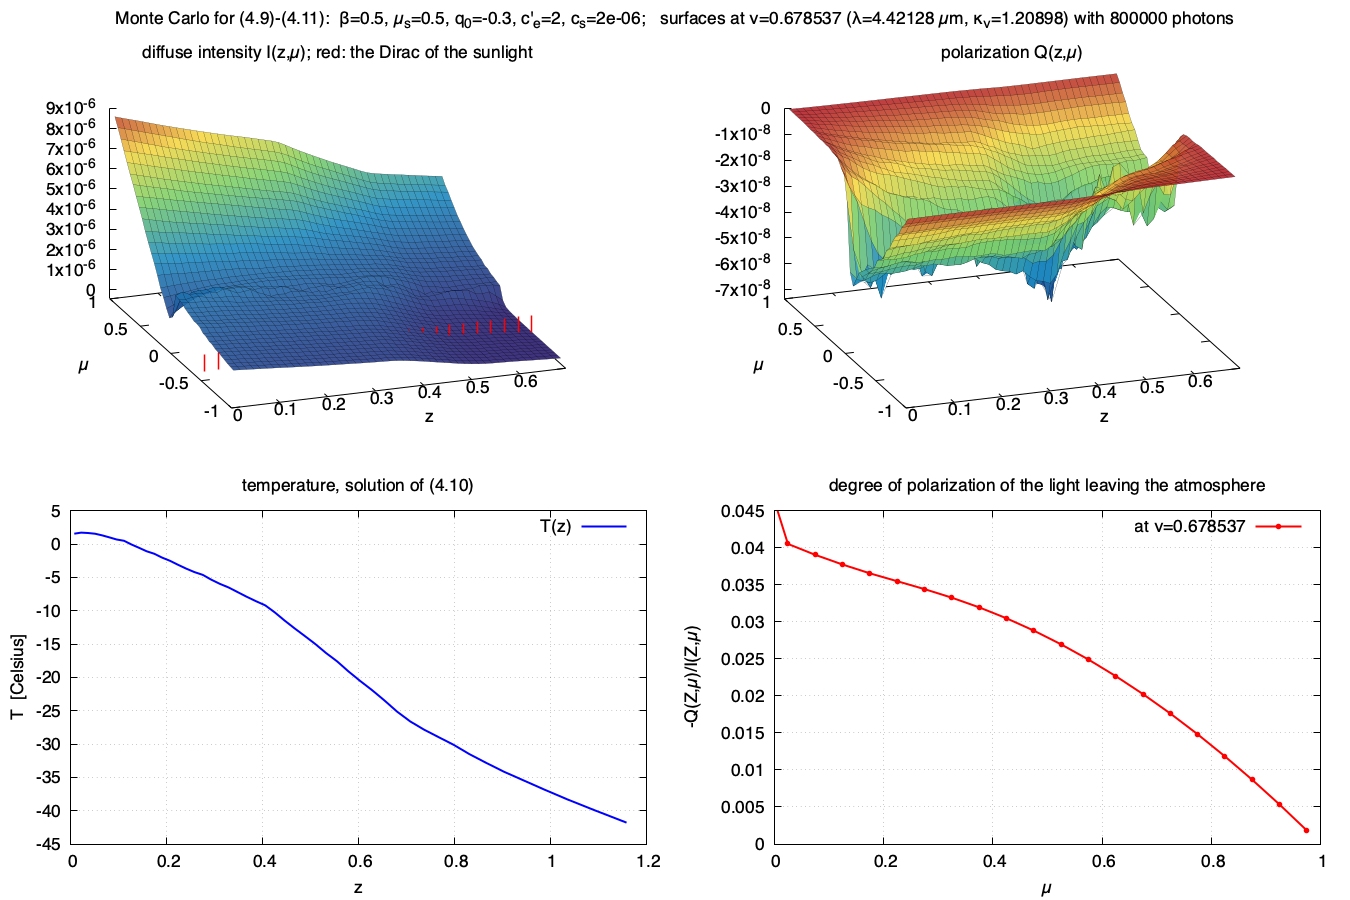
\includegraphics[width=\textwidth]{MCIQ4.png}
\caption{Monte Carlo solution. Top: the diffuse intensity $I(z,\mu)$ --- the Dirac of the
sunlight is drawn apart, in red --- and the polarization $Q(z,\mu)$, at
$\lambda=4.42\,\mu$m. Bottom: the temperature, solution of \eqref{eq:fort0}, and the
degree of polarization $-Q/I$ of the light leaving the atmosphere.}\label{fig:sol}
\end{figure}

Figure~\ref{fig:sol} shows the solution. The temperature falls from $+1.5\,^\circ$C at the
ground to $-41.8\,^\circ$C at the tropopause, with a change of slope in the cloud. The
light which leaves the atmosphere is polarized by 4\% at grazing angles and not at all at
the vertical, a quantity obtained here without any closure hypothesis.

\paragraph{Effect of CO$_2$.} Multiplying $\kappa_\nu$ by $1.2$ in the band
$14$--$18\,\mu$m gives Table~\ref{tab:co2} and Figure~\ref{fig:co2}: the ground warms by
$0.97\,^\circ$C and the tropopause cools by $1.35\,^\circ$C, the signature of a greenhouse
gas. ISIF, run on the same $120$ points, gives $+0.93$ and $-1.31\,^\circ$C. The two
methods therefore agree on the signal to $0.2\,^\circ$C everywhere (right of
Figure~\ref{fig:co2}), better than they agree on $T$ itself, because the systematic part of
the discretization error cancels in the difference. The residual wiggle of the Monte Carlo
curve, $\pm0.1\,^\circ$C, is what remains of the statistical error in a difference of two
independent runs of $2.8\times10^8$ trajectories.

\begin{table}[htb]\centering
\begin{tabular}{rrrrr}\toprule
&\multicolumn{3}{c}{Monte Carlo}&ISIF\\\cmidrule(lr){2-4}\cmidrule(lr){5-5}
$z$ & $T$ without CO$_2$ & $T$ with CO$_2$ & $\Delta T$ & $\Delta T$\\\midrule
0.003 &    0.47 &    1.45 &  $+0.97$ &  $+0.93$\\
0.087 &  $-0.05$ &    0.90 &  $+0.95$ &  $+0.91$\\
0.178 &  $-2.25$ &  $-1.50$ &  $+0.75$ &  $+0.71$\\
0.275 &  $-5.05$ &  $-4.60$ &  $+0.45$ &  $+0.47$\\
0.381 &  $-8.66$ &  $-8.29$ &  $+0.37$ &  $+0.18$\\
0.500 & $-14.65$ & $-14.60$ &  $+0.04$ &  $-0.02$\\
0.636 & $-22.42$ & $-22.44$ &  $-0.02$ &  $-0.19$\\
0.800 & $-29.89$ & $-30.46$ &  $-0.57$ &  $-0.48$\\
1.027 & $-37.14$ & $-38.11$ &  $-0.97$ &  $-1.00$\\\bottomrule
\end{tabular}
\caption{Temperature in $^\circ$C versus altitude, without and with the 20\% increase of
$\kappa_\nu$ in the CO$_2$ band, on the $120$ point grid; last column, the same difference
computed by ISIF.}\label{tab:co2}
\end{table}

\begin{figure}[htb]\centering
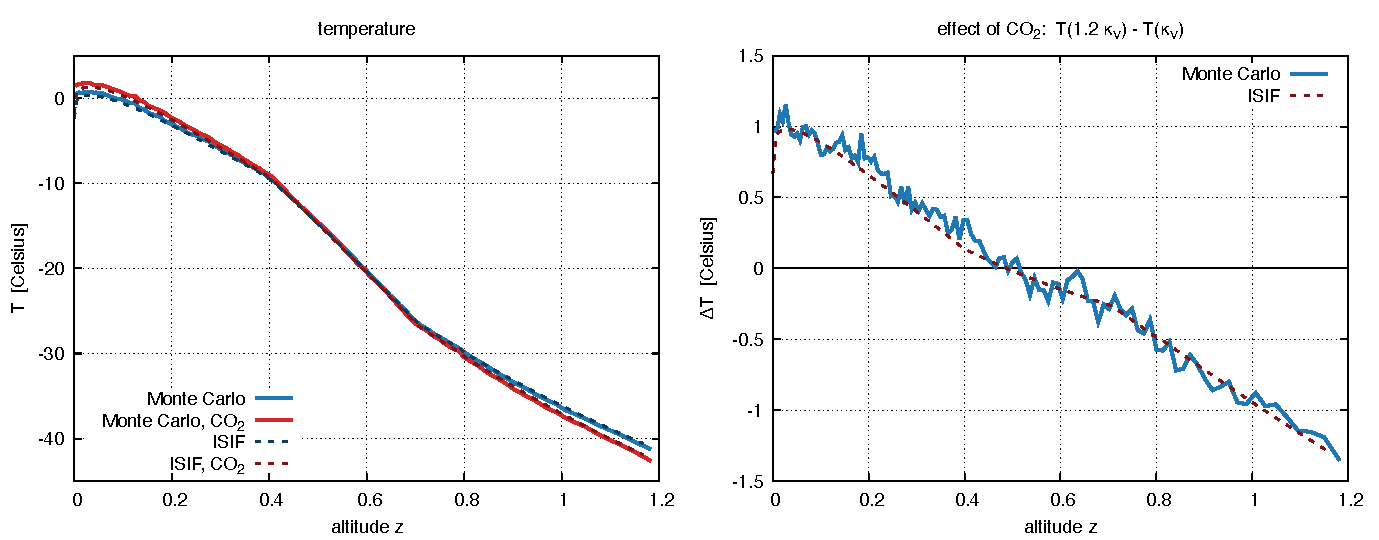
\includegraphics[width=\textwidth]{compareISIF2MC.pdf}
\caption{The two methods on the same $120$ point grid, with and without the increase of
$\kappa_\nu$ in the CO$_2$ band. Left, the temperatures, nearly superposed; the first node
of ISIF carries a boundary oscillation ($-2.3\,^\circ$C against $-0.1$ at the next node).
Right, the effect of CO$_2$ alone, on which the two methods agree to
$0.2\,^\circ$C.}\label{fig:co2}
\end{figure}

\paragraph{Cost.} The three methods on the same problem --- 554 frequencies, the CO$_2$
case, 25 temperature iterations --- on an Apple M4 Pro:
\begin{center}\small
\begin{tabular}{lrr}\toprule
& 49 cells & 119 cells\\\midrule
discrete ordinates, \texttt{SNIQ4.cpp} (64 directions) & 0.64 s & 1.65 s\\
ISIF, \ISIF & 1.06 s & 5.96 s\\
Monte Carlo, \MC\ ($2\cdot10^4$ photons per frequency) & 47 s & 102 s\\\bottomrule
\end{tabular}
\end{center}
The discrete ordinates solver needs $9.4$ source iterations per frequency and per
temperature iteration at the tolerance $10^{-8}$; 64 directions give the ground temperature
to $0.005\,^\circ$C, 32 to $0.07\,^\circ$C. It is the fastest of the three, and the more so
as the mesh is refined, its cost being $O(nN_z)$ against the $O(N_z^2)$ of the convolutions
of ISIF; the three give the same temperature, Figure~\ref{fig:three}. The Monte Carlo is not competitive in speed on this one dimensional problem; its
interest is elsewhere: it needs neither the closure by the four moments $J_0,J_2,K_0,K_2$,
nor the exponential integrals $\E_n$, nor the fact that the kernel is a polynomial in
$\mu^2$. A phase matrix of any shape, a non stratified geometry or a non grey ground would
be taken unchanged, and the frequencies are independent, hence trivially parallel.

\begin{figure}[htb]\centering
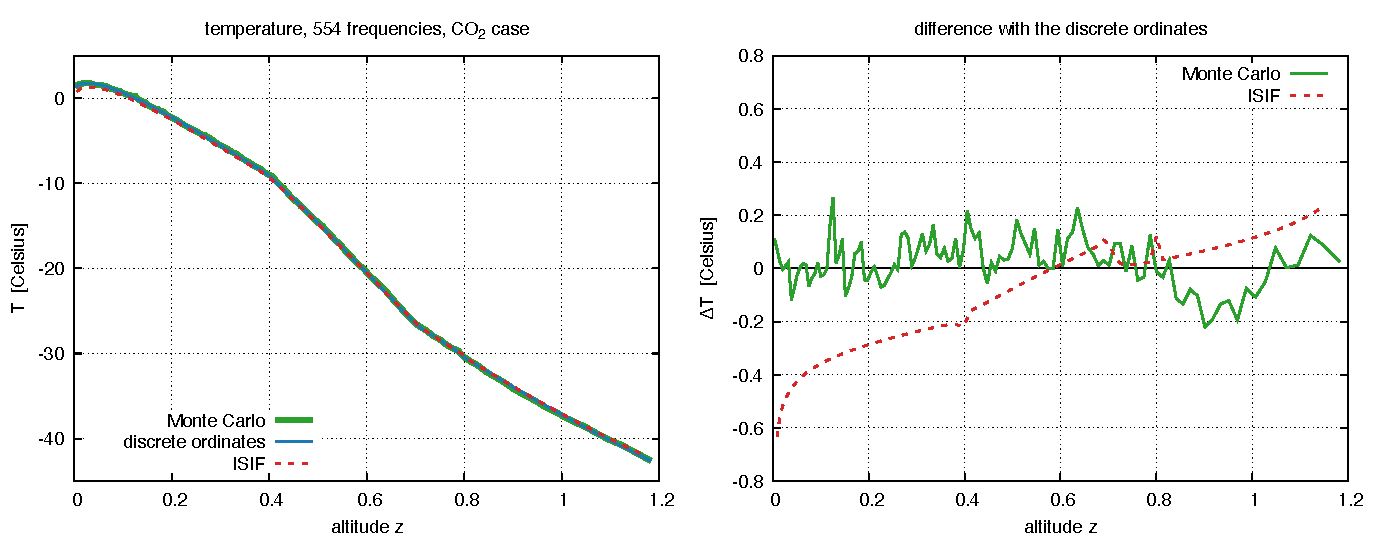
\includegraphics[width=\textwidth]{compare3methods.pdf}
\caption{The three methods on the same $119/120$ point grid, CO$_2$ case. Left, the
temperatures: indistinguishable at this scale. Right, the difference with the discrete
ordinates, taken as reference because it is the smooth and grid converged one. The Monte
Carlo oscillates about zero without any trend --- statistical noise, which decreases like
$N^{-1/2}$ --- at most $0.27\,^\circ$C, $0.09\,^\circ$C r.m.s.; ISIF departs smoothly and
systematically, $-0.6\,^\circ$C at the ground, $+0.2\,^\circ$C at the tropopause, at most
$0.63\,^\circ$C and $0.24\,^\circ$C r.m.s.}\label{fig:three}
\end{figure}

\paragraph{Use.} \texttt{g++ -O3 -std=c++17 -o MCIQ4 MCIQ4.cpp}, then \texttt{./MCIQ4}
with the optional arguments \texttt{N=} (photons per frequency and per iteration),
\texttt{iter=}, \texttt{nuplot=} (frequency of the surfaces), \texttt{Nplot=} (photons for
that frequency on the last sweep, $Q$ being noisier than $I$), \texttt{Nmu=},
\texttt{seed=}, \texttt{plot=0}. It writes \texttt{MCIQ4\_T.txt} ($T$ and the
$\nu$-integrals of $J_0,K_0$), \texttt{MCIQ4\_Jnu.txt} (the four moments at
\texttt{nuplot}), \texttt{MCIQ4\_I.txt} (the surfaces), \texttt{MCIQ4\_exit.txt} (the
emerging intensities) and the gnuplot script \texttt{MCIQ4.gp} of Figure~\ref{fig:sol}.

\section*{Acknowledgement}
The programs described here --- the Monte Carlo solver \MC\ and the discrete ordinates
solver written to verify it --- together with the figures and this memo, were produced by
Claude Code (Anthropic, model Opus~5), from the equations of Chapter~4 and the existing
ISIF program \ISIF.

\begin{thebibliography}{9}\small
\bibitem{hammersley} J.~M. Hammersley and D.~C. Handscomb, {\em Monte Carlo Methods},
Methuen, London, 1964.
\bibitem{spanier} J.~Spanier and E.~M. Gelbard, {\em Monte Carlo Principles and Neutron
Transport Problems}, Addison-Wesley, Reading, 1969.
\bibitem{marchuk} G.~I. Marchuk, G.~A. Mikhailov, M.~A. Nazaraliev et al., {\em The Monte
Carlo Methods in Atmospheric Optics}, Springer Series in Optical Sciences 12, Springer,
Berlin, 1980.
\bibitem{mayer} B.~Mayer, {\em Radiative transfer in the cloudy atmosphere}, EPJ Web of
Conferences, 1 (2009), pp.~75--99.
\bibitem{chandra} S.~Chandrasekhar, {\em Radiative Transfer}, Dover, New York, 1960.
\bibitem{stamnes} K.~Stamnes, S.-C. Tsay, W.~Wiscombe and K.~Jayaweera, {\em Numerically
stable algorithm for discrete-ordinate-method radiative transfer in multiple scattering and
emitting layered media}, Applied Optics, 27 (1988), pp.~2502--2509.
\bibitem{lewis} E.~E. Lewis and W.~F. Miller, {\em Computational Methods of Neutron
Transport}, Wiley, New York, 1984.
\bibitem{modest} M.~F. Modest, {\em Radiative Heat Transfer}, 3rd ed., Academic Press,
Oxford, 2013.
\end{thebibliography}

\end{document}
